\chapter{Background}
\label{cha:background}

In this chapter, we provide an overview of the main concepts, paradigms and technologies that are relevant for the purpose of this work.
We start by introducing the concept of \textbf{Public Cloud Providers} and the \textbf{Multi-Cloud paradigm}.
We then provide a brief overview of \textbf{Kubernetes}, in particular focusing on the concept of \textbf{Kubernetes as a platform} and the \textbf{Helm} package manager.
After that, \textbf{Krateo PlatformOps}, an open-source Kubernetes-based platform that is a fundamental part of our system, is introduced.
We also deemed valuable to provide an overview of the existing works in the field of \textbf{multi-cloud resource management} to highlight recurrent patterns and design choices.
Finally, the \textbf{GreenOps landscape} is introduced, focusing on the the \textbf{Computational Sustainability} initiatives by Public Cloud Providers and on \textbf{carbon-aware systems for resource management}. 

\section{Public cloud providers}

The Cloud Computing definition by the National Institute of Standards and Technology (NIST) \cite{nist_cloud_computing} states that ``\textit{Cloud Computing is a model for enabling ubiquitous, convenient, on-demand network access to a shared pool of configurable computing resources (e.g., networks, servers, storage, applications, and services) that can be rapidly provisioned and released with minimal management effort or service provider interaction}" \cite{nist_cloud_computing}.
\textbf{Public Cloud Providers} or Cloud Service Providers (CSPs) are companies that have as their core business the provisioning of cloud computing services. 
These services, which are growing in number and complexity over time, range from computing resources to storage, networking, databases, machine learning, and more. 
Public cloud is a deployment model that allows organizations to consume cloud services without having to build and maintain their own physical infrastructure (e.g., private cloud), therefore reducing capital expenditure (CapEx) and shifting to an operational expense model (OpEx). 
The public cloud model is actually a multi-tenant environment where physical resources maintained and operated by the cloud provider are shared among multiple customers (tenants) with the means of virtualization and isolation techniques.
These resources are offered in the form of various services at different levels of abstraction (e.g., Infrastructure as a Service, Platform as a Service, Software as a Service) and are provided on-demand on a pay-as-you-go basis.
%Doing so requires public cloud provider to leverage paradigm and technique which were known in the industry well before the advent of cloud computing: virtualization and isolation.
Currently, as of 2024, the public cloud market is dominated by three main hyperscalers: \textbf{Amazon Web Services (AWS)}, \textbf{Microsoft Azure}, and \textbf{Google Cloud Platform (GCP)}.
An hyperscaler is generally a company (Cloud Service Provider) that operates a data center infrastructure at a massive scale and is able to provide cloud services to a global audience.
Figure \ref{fig:pcp} shows the worldwide market share of leading cloud infrastructure service providers as of Q3 2024 \cite{statista_cloud_market_share}.

\begin{figure}[htb]
    \centering
    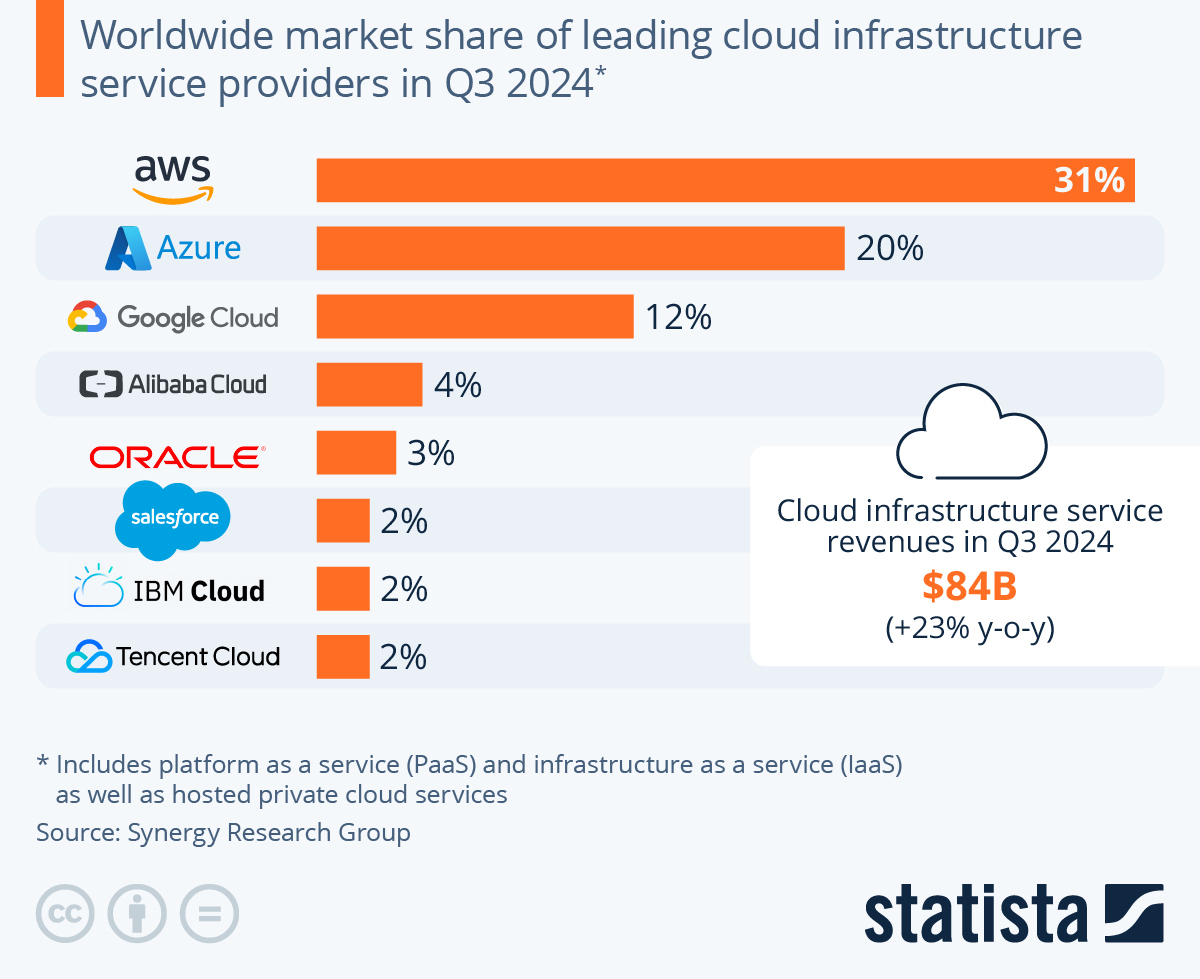
\includegraphics[width=0.75\linewidth]{images/pcp.jpeg}
    \caption{Worldwide market share of leading cloud infrastructure service providers as of Q3 2024 \cite{statista_cloud_market_share}}
    \label{fig:pcp}
\end{figure}
  
\subsection{Cloud Regions and Availability Zones}

With the term \textbf{cloud region}, cloud providers refer to a geographical area where they have one or more data centers.
Cloud providers usually further divide regions into availability zones (AZs) which main purpose is to provide high availability and fault tolerance.
For the purpose of this work, we will consider the concept of \textbf{cloud region} as the primary unit of deployment of cloud resources.
Usually, by cloud providers design choice, each cloud region supports only a subset of the available cloud services and instance types.
We could safely assume that our targeted workload specifications are quite standard and therefore can be scheduled on any cloud region.
As of late 2024, the three major cloud service providers have established extensive global infrastructures.
Table \ref{tab:cloud_regions_azs} shows the number of regions and availability zones (AZs) for each provider as of Q4 2024 - Q1 2025
\cite{statista_cloud_regions} \cite{aws_infrastructure}.
We must note that the number of regions and availability zones is constantly changing as cloud providers are expanding their global infrastructure.

\begin{table}[H]
    \centering
    \begin{tabular}{|l|c|c|}
    \hline
    \textbf{Cloud Provider} & \textbf{Regions} & \textbf{Availability Zones} \\
    \hline
    Amazon Web Services (AWS) & 36 & 114 \\
    \hline
    Microsoft Azure & 33 & 93 \\
    \hline
    Google Cloud Platform (GCP) & 40 & 121 \\
    \hline
    \end{tabular}
    \caption{Number of Cloud Regions and Availability Zones by Provider as of 2024 \cite{statista_cloud_regions}}
    \label{tab:cloud_regions_azs}
\end{table}

We must also note that each cloud provider has a different number of regions and zones and also different naming conventions for them.
There is no standardization nor a convention in the industry for this and cloud providers have chosen their own naming schemes.
For instance, a region located in London is called ``\textit{eu-west-2}'' in AWS, ``\textit{uk-west}'' in Azure and ``\textit{europe-west2}'' in GCP.
This detail must be taken into account when designing and implementing a multi-cloud system.
For what concerns the geo-distribution of cloud regions, as an example, Figure \ref{fig:azure_data_centers} shows the location of \textbf{Azure cloud data centers} around the world and the country Grid Carbon Intensity as reported by Electricity Maps (year 2024) \cite{electricity_maps}.
Data center coordinates are retrieved by an Azure CLI command dump \cite{azure_data_centers_information} and plotted on a map using the Natural Earth dataset \cite{naturalearthdata}.

\begin{figure}[htb]
    \centering
    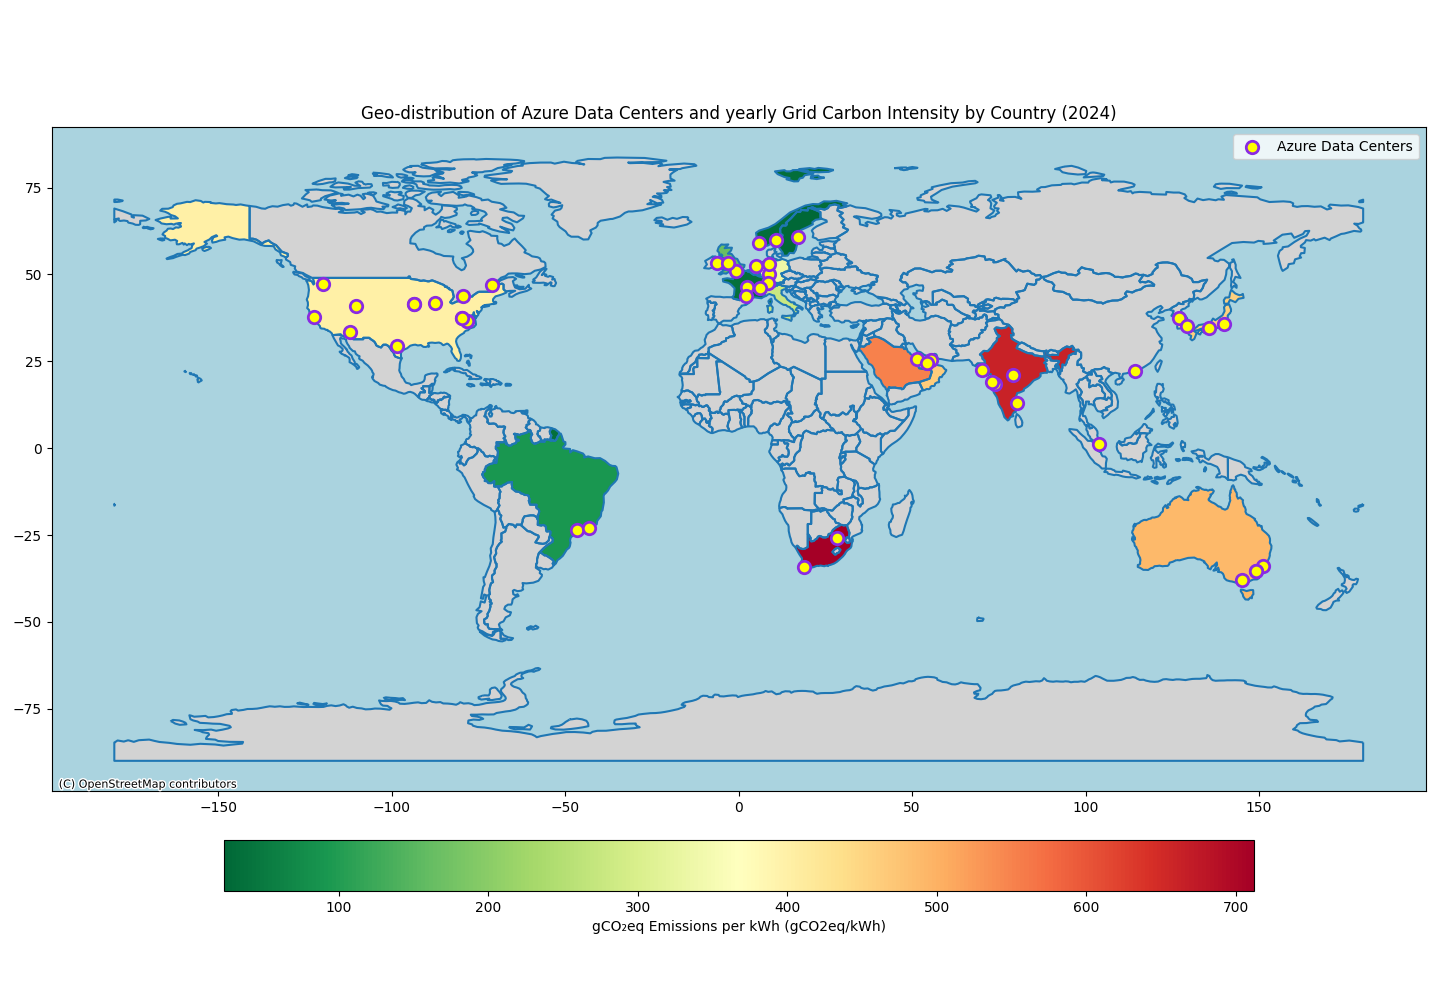
\includegraphics[width=1\linewidth]{images/azure_data_centers.png}
    \caption{Geo-distribution of Azure data centers with country Grid Carbon Intensity}
    \label{fig:azure_data_centers}
\end{figure}

\subsection{Multi-cloud paradigm}

The multi-cloud paradigm refers to the strategic utilization of cloud services from multiple public cloud providers within a single, heterogeneous architecture. 
This approach allows organizations to distribute workloads, applications, and data across multiple public cloud providers \cite{google_multicloud}.
On the other hand, the hybrid cloud paradigm refers to utilization of both public cloud services and on-premises infrastructure (private cloud).
The multi-cloud strategy is often adopted by organizations to \textbf{avoid vendor lock-in}, \textbf{increase redundancy}, \textbf{increase flexibility} and \textbf{optimize costs} \cite{google_multicloud}.
For what concern flexibility and optimization, a multi-cloud strategy allows an organization to select the best service on a case-by-case basis, leveraging the strengths of each provider.
Moreover, single point of failure weaknesses are mitigated by distributing workloads or critical services across multiple providers.
It could even be the case that, for the end user, the choice of the cloud provider for a service is transparent meaning that the organization itself (or the system) is the one that decides which cloud provider to use for a specific service based on some criteria.
Vendor lock-in can be avoided by designing applications to be \textbf{cloud-agnostic} and by leveraging open-source technologies (e.g., Kubernetes) and standards \cite{google_multicloud}.
If an application is designed to be cloud-agnostic, it can be relatively easily migrated from one cloud provider to another.
Multi-cloud is a strategy that might be more difficult to implement compared to a single cloud strategy but the long-term benefits are significant.
\textbf{Challenges} and \textbf{disadvantages} are also present in a multi-cloud strategy \cite{google_multicloud}.
As a matter of fact it can be safely said that \textbf{complexity in the overall infrastructure management is increased}.
Another challenge is the \textbf{integration of services} across different cloud providers.
An additional consideration could be done in terms of security: a multi-cloud strategy can \textbf{increase the attack surface} of an organization, therefore security measures must be carefully implemented.
\newline
For the purpose of this work, adopting a multi-cloud strategy is beneficial for several reasons.
First and foremost, \textbf{user-centric flexibility} is achieved bringing the benefits described above.
If a user or organization has a preference for a specific cloud provider, the system can be configured to use only that provider or a specific subset of providers.
Secondly, the system can be designed to be \textbf{cloud-agnostic}, meaning that the choice of the cloud provider is transparent to the end user. 
With some specific configurations, the subset of providers to be used can be decided by the system itself based on some criteria.
Currently, as described in section \ref{sec:scheduling_outcome_policy}, the user can specify a subset of cloud providers (among the 3 major ones) to be used for the deployment of resources.
Finally, in theory, since different cloud providers have data centers in various locations around the world, some low-carbon regions might be available only on a specific cloud provider and this could be leveraged for the deployment of resources.

\section{Kubernetes}

Kubernetes is an open-source platform for automating the orchestration of containerized applications.
It is widely used in the industry and became the \textbf{de-facto standard for container orchestration}.
An extensive description of Kubernetes is out of the scope of this thesis but it is deemed necessary to provide a brief overview of the main concepts of Kubernetes that are relevant for the purpose of this work.
Figure \ref{fig:kubernetes_architecture} shows the Kubernetes architecture as described by the Cloud Native Computing Foundation (CNCF) \cite{kubernetes_cnfc}.

\begin{figure}[htb]
    \centering
    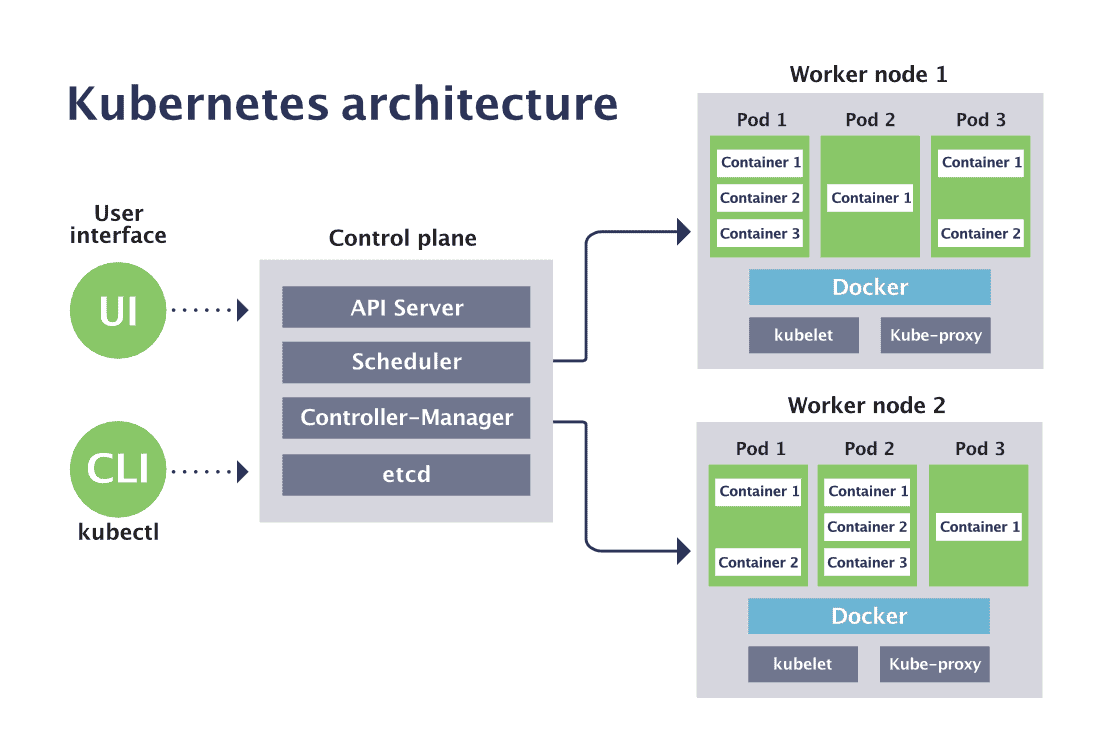
\includegraphics[width=1\linewidth]{images/kubernetes-architecture-diagram.png}
    \caption{Kubernetes architecture by CNCF \cite{kubernetes_cnfc}}
    \label{fig:kubernetes_architecture}
\end{figure}

The main components of Kubernetes are:
\begin{itemize}[itemsep=0.2pt, topsep=1pt]
    \item[$\bullet$] \textbf{Kubernetes API server}: the central component that manages the Kubernetes cluster. It exposes the Kubernetes API and is responsible for validating and mutating data related to Kubernetes objects before persisting them in the cluster state.
    \item[$\bullet$] \textbf{etcd}: a key-value store used to store the cluster state.
    \item[$\bullet$] \textbf{Kubernetes controller manager}: a daemon that embeds the core control loops shipped with Kubernetes.
    \item[$\bullet$] \textbf{Kubernetes scheduler}: a component that assigns Pods to nodes.
    \item[$\bullet$] \textbf{Kubelet}: an agent that runs on each node in the cluster. It makes sure that containers are correctly running in Pods.
    \item[$\bullet$] \textbf{Kubernetes proxy}: a network proxy that runs on each node in the cluster. It maintains network rules and it is responsible for routing network traffic.
    \item[$\bullet$] \textbf{Container runtime}: the software that is responsible for running containers on the Node (in this case represented by Docker but other runtimes like containerd are supported).
\end{itemize}

The first four components are the main control plane components of Kubernetes while the last three are the main components of each worker node in the cluster.
It must be noted that in our system we are not extending the Kubernetes scheduler as described for instance in the works described in section \ref{sec:low_carbon_k8s_scheduler} and \ref{sec:microsoft_carbon_aware_k8s}, since we are not dealing with the scheduling of in-cluster resources (e.g., Kubernetes Pods) nor with the provisioning of entire Kubernetes clusters.
We are instead focusing on the \textbf{management of external resources on cloud providers} (only VMs in this first iteration), leveraging Kubernetes as a control plane for the management of these resources.
As described in the following section, our focus will be on the Kubernetes API server and in particular on Kubernetes Admission Control.

\subsection{Kubernetes extendability}
\label{sec:kubernetes_extendability}

% https://www.cncf.io/blog/2022/06/15/kubernetes-operators-what-are-they-some-examples/

Kubernetes allows for the extension of its functionalities through the use of \textbf{Custom Resource Definitions (CRDs)} and \textbf{Kubernetes Operators}, effectively adopting the so-called \textbf{Operator paradigm}.
Simply put, Custom Resource Definitions are a way to instruct Kubernetes to manage new resource types. 
They are a \textbf{schema} that defines the structure of the resource and the Kubernetes API server will validate the resource against the schema.
\textbf{Custom Resources (CRs)} are actually instances of the resources defined by CRDs and are managed by an Operator.
The Operator is a piece of software (controller) that is responsible for managing the lifecycle of the resources defined by the CRD.
Effectively the code of an Operator is usually deployed on the Kubernetes cluster in the form of a Deployment.
This concept is not much different of what actually happens for standard built-in Kubernetes resources which are however manged by built-in controllers (e.g., Deployment controller, ReplicaSet controller, part of Kubernetes controller manager).
An high-level overview of the Operator paradigm is depicted in Figure \ref{fig:operator_paradigm}.

\begin{figure}[H]
    \centering
    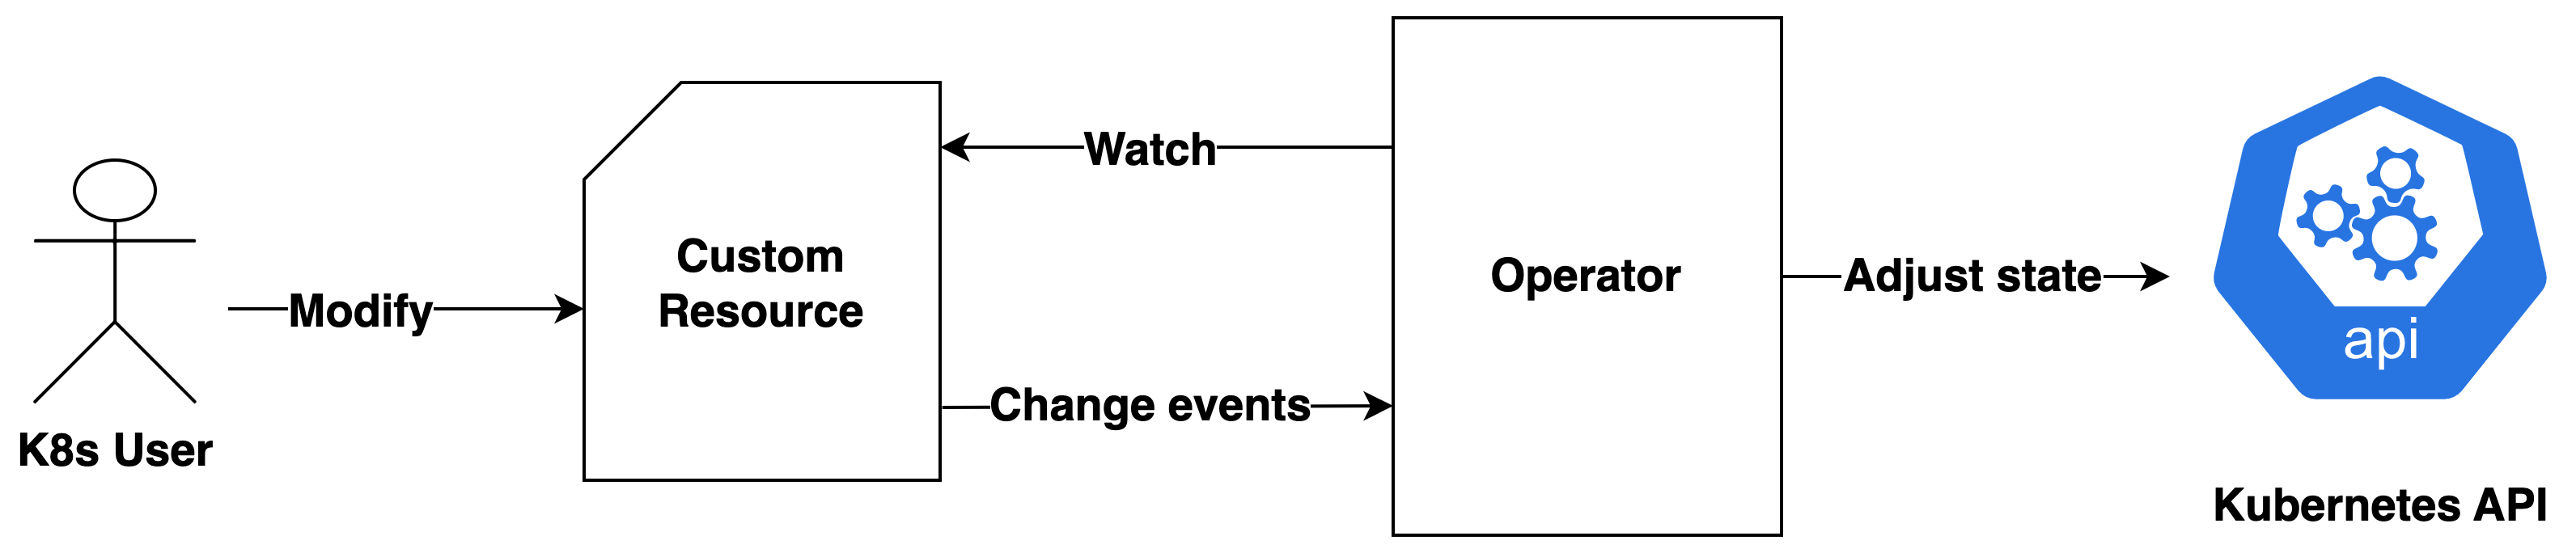
\includegraphics[width=1\linewidth]{images/opeartor_paradigm.png}
    \caption{Operator paradigm}
    \label{fig:operator_paradigm}
\end{figure}

\subsection{Kubernetes as a platform}

Recently, the paradigm of leveraging Kubernetes as a platform to manage external resources has become more and more popular.
Therefore, Kubernetes use cases have expanded beyond the management of containerized applications to the management of any desired resource on any infrastructure.
The idea is to \textbf{represent external resources as Kubernetes objects} and leverage Kubernetes' declarative paradigm and robust API to achieve unified and efficient infrastructure management.
This approach can be exemplified by the public cloud providers' operators which extend Kubernetes to manage their cloud resources as described in section \ref{sec:cloud_providers_operators}.

For instance, Config Connector is a Kubernetes operator developed by Google Cloud that allows to configure numerous Google Cloud services and resources using Kubernetes tooling and APIs \cite{gcp_config_connector}.
The idea general idea is that organizations might have to deal with a \textbf{heterogeneous infrastructure} composed of different cloud providers and on-premises resources. 
By \textbf{unifying infrastructure management under Kubernetes}, complexity is reduced and velocity is increased because the same tools and APIs can be used to manage all the resources in a consistent way \cite{gcp_config_connector}.


% https://aws.amazon.com/it/blogs/containers/kubernetes-as-a-platform-vs-kubernetes-as-an-api-2/

\subsection{Helm}

Helm is a \textbf{package manager} for Kubernetes. Therefore with Helm it is possible to define, install and manage Kubernetes applications in a simpler way compared to a manual management of Kubernetes resources manifests \cite{helm}.
Helm is a graduated project in the CNCF and it is the de-facto standard for Kubernetes package management.
The key concept is the \textbf{Helm chart}, which is a collection of files that describe a related set of Kubernetes resources. 
These files are mainly of two types: templates and values.
The \textbf{templates} are Kubernetes manifest files that are rendered by Helm's \textbf{powerful templating engine}. 
The \textbf{values} are the set of variables that are used to render the templates.
Upon an Helm chart installation, Helm will render the templates ``injecting" the values and deploy the resources in the Kubernetes cluster. 
One major advantage that Helm provides is the complete management of the lifecycle of the resources.
As a matter of fact, Helm allows to easily \textbf{upgrade}, \textbf{rollback} and \textbf{uninstall} the Kubernetes resources deployed with a Helm chart reducing time and errors in such operations \cite{helm}. 
Without Helm, the user would have to deal with each single Kubernetes resource manifest file and manually apply changes to them.
Finally, users can benefit of Helm charts already developed by the community and leverage chart distribution within their organization using Helm repositories.

\section{Krateo PlatformOps}
\label{sec:krateo}

Krateo PlatformOps (Krateo) is an \textbf{open-source Kubernetes-based platform} that aims to provide a unified interface for managing any desired resource on any infrastructure \cite{krateo_docs}.
Krateo runs as a Kubernetes deployment inside a Kubernetes cluster but \textbf{acts as a control plane} even for resource external to the Kubernetes cluster.
The only requirement for this management is that the resources need to be logically descriptible using a YAML file which represents the desired state of the resources \cite{krateo_docs}.
% Platform engineering
% Developer platform: a unified environment providing tools, services, and infrastructure that enables teams to efficiently build, test, and deploy software without managing underlying complexity. This complexity is handled by the platform team.
% Recognized by Gartner. Gartner said ... by 2025 companies without a ... (cite)
Krateo is composed of three main parts:
\begin{itemize}[itemsep=0.2pt, topsep=1pt]
    \item[$\bullet$] Krateo Composable Operations
    \item[$\bullet$] Krateo Composable Portal
    \item[$\bullet$] Krateo Composable FinOps
\end{itemize}

For the purpose of this work, we will focus on the \textbf{Krateo Composable Operations} part, which is the core of the Krateo platform and is responsible for managing the lifecycle of resources in a Kubernetes cluster \cite{krateo_docs}.
Krateo Composable Operations is composed in turn by several components. 
Due to their core importance in our system, we will briefly describe the functionalities of the \textbf{Krateo core-provider} and the \textbf{Krateo composition-dynamic-controller} as described in Krateo official documentation (\cite{krateo_core_provider} and \cite{krateo_composition_dynamic_controller}).

\subsection{Krateo core-provider}

The Krateo core-provider, as its name suggests, is the core component of the Krateo platform.
It is a \textbf{Kubernetes operator} that has the duty of downloading and managing Helm charts. 
It first checks for the existence of a file named \textit{values.schema.json} in the chart folder and uses it to generate a Kubernetes Custom Resource Definition (CRD), accurately representing the possible values that can be expressed for the installation of the chart \cite{krateo_core_provider}.
The file \textit{values.schema.json} is a JSON schema that describes the structure of the \textit{values.yaml} file for the related Helm chart and it is considered a standard best practice for Helm charts. 
It basically provides a way to validate the \textit{values}.yaml file before the Helm chart is installed (i.e., to check if the values are in the correct format and if all the required values are present) \cite{krateo_core_provider}.
Therefore the file \textit{values.schema.json} could be useful in the context of DevOps practices and CI/CD pipelines but in the case of Krateo it is pivotal for the generation of the CRD.
In other words, the Krateo core-provider operator is responsible for deploying the Helm chart as a \textbf{native Kubernetes resource}, which allows for the management of the whole Helm chart lifecycle through Kubernetes APIs \cite{krateo_core_provider}.
As a matter of fact, out of the box, Kubernetes does not provide a way to manage Helm charts natively and the Krateo core-provider is one tool that allows to do so.
The Kubernetes Custom Resource Definition introduced by the Krateo core-provider is called \textbf{\textit{CompositionDefinition}}. 
It is a CRD that represents the Helm chart and its values (a Helm Chart archive (.tgz) with a JSON Schema for the values.yaml file) \cite{krateo_core_provider}.
Upon a CompositionDefinition manifest application to the Kubernetes cluster, the Krateo core-provider generates the CRD from the schema defined in the \textit{values.schema.json} file included in the chart. 
It then deploys an instance of the Krateo composition-dynamic-controller, setting it up to manage resources of the type defined by the CRD \cite{krateo_core_provider}.
Therefore, this is an example of the Operator paradigm described in section \ref{sec:kubernetes_extendability} where the Krateo core-provider is the Operator and the CompositionDefinition is the Custom Resource Definition.

\subsection{Krateo composition-dynamic-controller}

The Krateo composition-dynamic-controller is the Kubernetes operator that is instantiated by the Krateo core-provider to manage the specific Custom Resources whose Custom Resource Definition is generated by the core-provider.
In practice, when a Custom Resource (CR) is created, the specific instance of composition-dynamic-controller checks if a Helm release associated with the CR already exists in the cluster \cite{krateo_composition_dynamic_controller}. 
If this is not the case, it performs an \textit{helm install} operation using the values specified in the CR to create a new Helm release. This will practically deploy all the resources defined in the Helm chart using \textbf{Helm's templating engine}.
This feature is particularly important in the context of the system described in this thesis and in particular for multi-cloud resource management as explained in section \ref{sec:krateo_integration}.
However, if the Helm release does already exist, it instead executes an \textit{helm upgrade} operation, updating the release's values with those specified in the CR, effectively updating the resources in the cluster.
This mechanism will be leveraged as well for a particular feature  of our system (i.e., ``waiting logic'') described in section \ref{sec:scheduling_time_waiting_logic}.
Finally, when the CR is deleted from the cluster, the instance of the composition-dynamic-controller performs an \textit{helm uninstall} on the release, removing all the resources defined in the Helm chart from the cluster \cite{krateo_composition_dynamic_controller}. \\
It must be said that Krateo composition-dynamic-controller has a set of additional features that are not described in this work such as multi-version support.
The architecture of the Krateo core-provider and Krateo composition-dynamic-controller is depicted in Figure \ref{fig:krateo_core_provider}, as described and depicted in \cite{krateo_core_provider}.

\begin{figure}[htb]
    \centering
    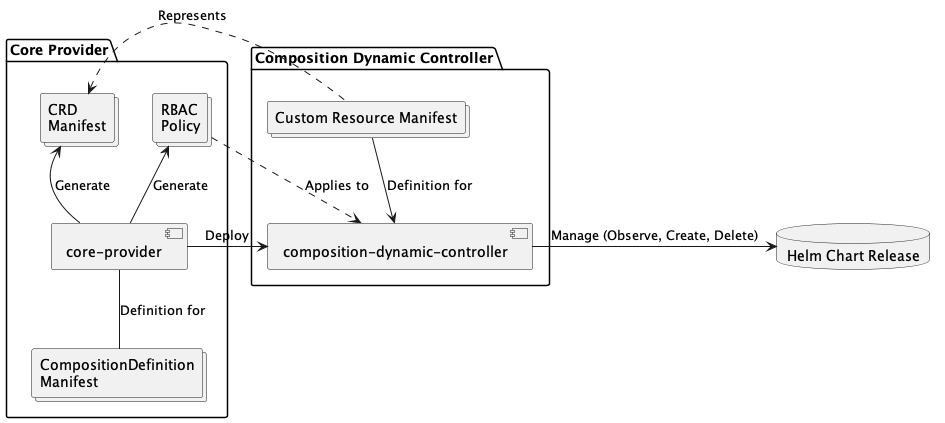
\includegraphics[width=1\linewidth]{images/kraeto_core_provider.png}
    \caption{Krateo core-provider and composition-dynamic-controller architecture \cite{krateo_core_provider}}
    \label{fig:krateo_core_provider}
\end{figure}

\section{Multi cloud resource management}
\label{sec:multi_cloud_resource_management}

The idea of a \textbf{dynamic management of workloads leveraging a multi-cloud paradigm} is not new. In this section we will provide an overview of some of the existing works in the literature that have tackled the problem of multi-cloud resource management.

\subsection{Dynamic Virtual Machine placement}
The work of Simarro et al. \cite{Simarro_2011} back at the dawn of cloud computing (2011) proposed a multi-cloud architecture for the dynamic placement of Virtual Machines (VMs).
The main objective of the system was cost optimization but this paradigm provides reliability and flexibility as well.
The scheduling part is comprised of a ``\textbf{cloud broker}" that is responsible for VM placement \textbf{transparent to users} providing a single uniform interface to the cloud resources.
Users can provide to the system a ``\textbf{service description template}'' to specify the number of VMs to provision and some constraints.
The cloud broker architecture is composed of two major components: the \textbf{scheduler} and the \textbf{cloud manager} \cite{Simarro_2011}. The former is responsible for placement decision across multiple cloud providers, while the latter is responsible for the actual management of the VMs in the cloud providers. More precisely, the cloud manager is represented by the OpenNebula (ONE) virtual infrastructure manager \cite{Simarro_2011}.
OpenNebula is an open-source platform that aims to provide a unified management interface for multiple virtualization technologies and cloud providers \cite{open_nebula}.

\subsection{Cloud service brokers}
A CSB is a system that acts as an \textbf{intermediary} between cloud service providers and consumers, providing a \textbf{unified interface} to manage cloud resources across multiple providers \cite{Wadhwa_2013}.
Cloud service brokers (CSBs) were described and categorized by Wadhwa et al. \cite{Wadhwa_2013} in their work of 2013.
The emerging market of cloud computing led to the proliferation of cloud services and providers, and by consequence the need for mechanisms to manage costs, capacity and resources \cite{Wadhwa_2013}. 
\newline

An interesting CSB example in the literature is the \textbf{STRATOS} system by Pawluk et al. proposed in 2012. The work can be considered a pioneer in the field of multi-cloud resource management since it can be framed in the first years of cloud computing \cite{STRATOS} but the proposed paradigms and concepts are relevant today.
STRATOS tried to \textbf{avoid the assumption of resource homogeneity} and represented an initial attempt to provide a ``\textbf{cross-cloud resource provisioning}'' system \cite{STRATOS}.
The proposed architecture enables the specification of high-level objectives that can be assessed in a standardized manner across different providers. The decision-making process is fully automated, shifting the decision point from deployment to runtime \cite{STRATOS}.
Users first submit a topology document, triggering the Cloud Manager to communicate with the Broker for topology instantiation. The Broker (implemented in Java) then conducts the initial resource acquisition decision (RAD), optimizing the allocation of resources across multiple providers (configured beforehand) \cite{STRATOS}.
Experiments indicate that distributing workloads across different cloud providers can reduce the overall cost of the topology. The approach taken by the authors primarily focuses on two objectives: \textbf{cost efficiency} and \textbf{avoiding vendor lock-in}. The application environment was deployed on public cloud platforms, specifically AWS and Rackspace \cite{STRATOS}.
\newline

[TO BE ADDED]
A Kubernetes 'Bridge' operator between cloud and external resources
% https://arxiv.org/abs/2207.02531

\subsection{AI-based resource management in cloud computing}
\label{sec:ai_based_resource_management}

More recent works have focused on the development of systems that leverage AI techniques for the optimization of resource management in cloud computing environments.

The work of 2022 by Khan et al. \cite{KHAN2022103405} provides a comprehensive review of the state of the art in the field of machine learning (ML)-centric resource management in cloud computing.
Although this works focuses on the cloud provider side (\textbf{resource management in data centers}), it provides some interesting insights that can be leveraged also at different levels of the cloud computing stack.
The authors highlight the fact that traditionally, only static policies were used for resource management in cloud computing, but the advent of ML techniques has enabled the development of more dynamic and adaptive resource management systems \cite{KHAN2022103405}. \newline
% maybe add some more insights from this work

Tuli et al. in their work of 2021 \cite{TULI2022111124} propose a system named \textbf{HUNTER} which stands for ``Holistic resoUrce
maNagemenT technique for Energy-efficient cloud computing using aRtificial intelligence''. 
In particular, in this work, tasks are modeled as \textbf{containers instances}.
For the purpose of this thesis, we can describe how this system was implemented from a infrastructural point of view.
The system is composed of four main components \cite{TULI2022111124}:
\begin{itemize}[itemsep=0.2pt, topsep=1pt]
    \item[$\bullet$] \textbf{Cloud Workload Management Portal}: a web-based portal that allows users to submit their workloads and specify the requirements (SLA constraints, QoS constraints, etc.).
    \item[$\bullet$] \textbf{Workload Manager}: a component that is responsible for the processing of incoming workloads.
    \item[$\bullet$] \textbf{Cloud Broker}:  the component that is responsible for the allocation of resources to cloud worker nodes
    \item[$\bullet$] \textbf{Cloud Hosts}: set of cloud worker nodes (in the form of both private and public cloud)
\end{itemize}
The Cloud Broker is the core of the system and is further divided into three sub-managers: Service Manager, CDC Manager, and Resource Manager.
The Service Manager is responsible for SLAs and QoS constraints, the CDC Manager is responsible for the actual allocation (provisioning) and migration of resources to cloud worker nodes and resource monitoring and the Resource Manager is responsible for the scheduling of tasks and contains the actual sustainability models (energy, thermal, cooling.) \cite{TULI2022111124}.

\subsection{Policy-driven resource management systems}

García García et al. (2014) propose \textbf{Cloudcompaas} \cite{GARCIAGARCIA20141}, a Service Level Agreement (SLA)-driven platform for dynamic cloud resource management, focusing on the automation of resource provisioning, scheduling, and monitoring
The aim of the work is to provide a SLA-aware Platform-as-a-Service platform for the entire management of cloud resource lifecycle \cite{GARCIAGARCIA20141}.
The targeted resource to be manages spans from IaaS to PaaS and SaaS.
Their approach leverage the WS-Agreement specification, a standard for SLA negotiation in web services, to define the SLA between the cloud provider and the cloud consumer \cite{GARCIAGARCIA20141}.
Leveraging this representation, they propose a SLA-driven architecture with three main components: the \textbf{SLA Manager}, the \textbf{Orchestrator}, and the \textbf{Infrastructure Connector} \cite{GARCIAGARCIA20141}.
The SLA Manager is the entry point for users and essentially builds and register agreements starting from the user requirements.
The Orchestrator, having a complete view of all the available cloud backends, performs the critical task of scheduling and resource allocation, considering the SLA constraints.
The Infrastructure Connector is the component that actually interacts with the cloud providers, performing the actual resource allocation and deallocation (provisioning and deprovisioning) \cite{GARCIAGARCIA20141}.
An interesting feature of the Infrastructure Connector is the ``configuration step'' in which arbitrary actions can be performed such as the \textbf{injection of a monitoring agent on a Virtual Machine}.
\newline

In the context of serverless computing environments, the work of 2021 by Mampage et al. \cite{9499407} proposes a deadline-aware dynamic resource management system.
The focus of the research is on both the provider and the consumer perspective, proposing a placement policy and ``dynamic resource management policy" that aims to minimize the cost of the provider while meeting the requirement of the consumer (i.e., the \textbf{deadline}) \cite{9499407}.
\newline


%[Policy-Based Cloud Management Through Resource Usage Prediction]
% https://link.springer.com/chapter/10.1007/978-3-319-13464-2_14

%---

% Optimizing Cost and Maximizing Profit for Multi-Cloud-Based Big Data Computing by Deadline-Aware Optimize Resource Allocation
% https://link.springer.com/chapter/10.1007/978-981-15-8469-5_3

\section{GreenOps landscape}

GreenOps is the abbreviation for ``\textbf{Green Operations}" and is the term used to describe an operational model that aims to integrate sustainable practices into an organization's digital operations, with a particular focus on cloud computing and data centers.
The interest in GreenOps has been growing in the last years due to the increasing awareness of the environmental impact of data centers and cloud infrastructures.
As a matter of fact according to various sources, the carbon footprint of data centers is [...]
The rising interest in the GreenOps ecosystem is also influenced by political and regulatory factors as the European Union's ambitious goals for the reduction of greenhouse gas emissions.
In particular, the \textit{Climate Neutral Data Centre Pact in Europe}, is an EU initiative which aims for making climate-neutral data centers by 2030 \cite{climate_neutral_data_centre_pact}.
Being the work of this thesis focused on the cloud ecosystem, we deem useful to cite the Technical Advisory Group (TAG) on Environmental Sustainability which is focused on the cloud-native sustainability landscape.
The TAG is part of the Cloud Native Computing Foundation (CNCF) and aims to provide guidance, standards, and best practices for the industry \cite{tag_env_sustainability}.

% https://hbr.org/2020/09/how-green-is-your-software
% https://www.usenix.org/publications/loginonline/slos-and-ghgs

\subsection{Green Software foundation}

Another pivotal actor in the GreenOps landscape is the Green Software Foundation.
The Green Software Foundation is a non-profit organization, part of the Linux Foundation, that aims to promote the development of green software and to provide a set of standards, tooling and best practices for the industry \cite{green_software_foundation}.
It is considered useful to provide a quick summary of the foundation's major projects that are relevant to the context of this work.

\subsubsection{Software Carbon Intensity Specification}

Software Carbon Intensity Specification (SCI) is a specification that aims to provide a standard way to measure the carbon intensity of software systems.
SCI is defined as a rate: the amount of carbon emissions per one unit of $R$ where $R$ is a functional unit for the software system (e.g., API call, new user, DB query, etc.) \cite{sci}.

The SCI can be defined as follows:
\[
SCI = C \times R = (O + M) \times R = ((E \times I) + M) \times R
\]

where:
\begin{itemize}[itemsep=0.2pt, topsep=1pt]
    \item[$\bullet$] $SCI$ is the Software Carbon Intensity
    \item[$\bullet$] $C$ is the carbon emissions
    \item[$\bullet$] $R$ is the functional unit
    \item[$\bullet$] $O$ is the operational emissions
    \item[$\bullet$] $M$ is the embodied emissions
    \item[$\bullet$] $E$ is the energy consumption
    \item[$\bullet$] $I$ is the carbon intensity
\end{itemize}

\subsubsection{Real Time Cloud}
\label{sec:real_time_cloud}

The Real Time Cloud project aims to provide a standard for real-time carbon emissions data reporting for cloud providers.
The goal is to provide real-time access to information about cloud region, PUE, WUE, carbon-free energy from the grid and from Cloud provider individual initiatives.
The concept is similar to FOCUS specification for FinOps but is at a very early stage and is not yet adopted by cloud providers as of 2025 \cite{real_time_cloud}.

%https://github.com/Green-Software-Foundation/real-time-cloud?tab=readme-ov-file

\subsubsection{Impact Framework}
\label{sec:impact_framework}

The Impact Framework is a flexible framework for measuring and reporting the environmental impact of software systems \cite{impact_framework}.
The core of the framework is represented by a \textbf{Manifest file} which is a YAML file that is used both for describing \textbf{calculation pipelines} and for storing the results of the calculations.
Pre-built plugins are available for the most common calculations (e.g., carbon intensity, energy consumption, etc.) but custom plugins can be developed as well \cite{impact_framework}.
A potential integration of this framework with our system is described in section \ref{sec:impact_framework_integration}.

%https://patterns.greensoftware.foundation/catalog/cloud/choose-region-closest-to-users
%[which patterns are used in our system]

\subsection{Computational Sustainability by Public Cloud Providers}

[TO BE FIXED] \newline

For the purpose of ths work, we assume that a cloud data center will likely rely on the same energy sources that characterize a specific geographical region.
Indeed, cloud data centers typically draw power from their local electrical grids, meaning their carbon emissions are closely tied to the energy mix of their specific geographical regions just like any other industrial facility.
For instance, if Finland's energy production is characterized by low carbon emissions, data centers located there are likely powered by clean energy sources. 
However, some public cloud providers may implement individual initiatives to enhance their access to renewable energy and by consequence to reduce their carbon footprints.
 

%what are they already doing
%improving energy efficiency by reducing their PUE
%(Power Usage Effectiveness (PUE) is the ratio of the total energy used by a data center to the energy used for computing.)

%what microsoft is already doing with alternative energy sources apart from grid

%https://blog.google/inside-google/infrastructure/data-centers-work-harder-sun-shines-wind-blows/

%Google CFE\%: “This is the average percentage of carbon free energy consumed in a particular location on an hourly basis, while taking into account the investments we have made in carbon-free energy in that location. This means that in addition to the carbon free energy that's already supplied by the grid, we have added carbon-free energy generation in that location”.
When selecting a Google Cloud region, the user can see the carbon-free energy percentage (CFE\%) for that region.

%usually big companies leverage financial instruments like PPAs to buy renewable energy therefore their emissions are not zero but they are offset by the renewable energy they buy.

As an example of the efforts made by public cloud providers in the field of carbon-aware computing, we can describe how Google has been working on carbon-aware computing for internal use. 
In particular, they exploit workload flexibility to shift when, where and how computing is done to reduce carbon emissions \cite{google_carbon_aware_computing}.
Some of the types of workloads they identified as flexible are: \textbf{video processing}, \textbf{training large-scale machine learning models}, \textbf{simulation pipelines}.
The main components they recognized to be necessary for carbon-aware computing are: accurate carbon intensity data, scalable infrastructures and migrations mechanisms \cite{google_carbon_aware_computing}.
Another important point is to adopt a \textbf{data-driven methodology}.
Indeed, at Google the total amount of work (computing) that needs to get done per day is quite predictable thanks to the large amount of data they can analyze to make predictions \cite{google_carbon_aware_computing}.

In section \ref{sec:carbon_metrics} we will briefly describe how public cloud providers are already providing carbon footprint data reports to their customers.

\section{Carbon-aware systems for resource management}

Having provided an overview of the existing works in the field of multi-cloud resource management and having introduced the GreenOps landscape, we now focus on the state of the art in the field of carbon-aware resource management.
In particular, implementation choices and design patterns that can be leveraged for the development of a carbon-aware resource management system will be discussed.
\newline

The work of 2023 by Sukprasert et al. named ``\textit{Spatiotemporal Carbon-aware Scheduling in the Cloud: Limits and Benefits}'' \cite{10.1145/3599733.3606301} is a comprehensive analysis on the limits and benefits of the employment of geographical shifting and time shifting for cloud workloads.
The authors highlight the fact that different workloads have different characteristics and therefore different degrees of flexibility. Those include, for instance: \textbf{execution deadlines}, \textbf{data protection laws}, and \textbf{latency requirements}. Therefore, carbon savings are constrained by a complex set of factors that need to be taken into account when designing a carbon-aware system \cite{10.1145/3599733.3606301}.
The following sections will present systems that have been developed by various research groups to tackle the problem of carbon-aware resource management in cloud computing environments.

%Bringing Carbon Awareness to Multi-cloud Application Delivery

\subsection{CASPER}

CASPER (Carbon-Aware Scheduling and Provisioning for Distributed Web Services) is a carbon-aware scheduling and provisioning system whose primary purpose is to minimize the carbon footprint of distributed web services \cite{Souza_2023}.
The system is defined as a multi-objective optimization problem that considers two factors: the \textbf{variable carbon intensity} and the \textbf{latency constraints} of the network \cite{Souza_2023}.
By evaluating the framework in real-world scenarios, the authors demonstrate that CASPER achieves significant reductions in carbon emissions (up to 70\%) while meeting application \textbf{Service Level Objectives (SLOs)}, highlighting its potential for practical implementation in large-scale distributed systems \cite{Souza_2023}.
The authors of CASPER highlight the importance of considering the workload characteristics such as memory state, \textbf{latency} and \textbf{regulatory constraints such as GDPR} \cite{Souza_2023}.
The system is not adopting time-shifting since it is dealing with web services that are by their nature non-stopping workloads. The architecture is tied to scheduling K8s resources inside K8s clusters and does not consider external resource management.
%https://github.com/carbonfirst/casper?tab=readme-ov-file
%[HOW is it deployed]

\subsection{CASPIAN}

A research on carbon-aware scheduling in Kubernetes environments was conducted by the authors of CASPIAN (A Carbon-aware Workload Scheduler in Multi-Cluster Kubernetes Environments) \cite{10786568}.
The proposed system leverages Multi Cluster App Dispatcher (MCAD), a multi-cluster management platform, to provision workloads over distributed Kubernetes clusters \cite{10786568}.
Caspian is a scheduling and placement controller which lives in a master cluster and interacts with the MCAD to provision workloads across multiple geographical distributed clusters \cite{10786568}.
In particular, two main components are described: the \textbf{carbon tracker} and the \textbf{scheduler}.
The carbon tracker is responsible for the periodic collection of carbon intensity data along with worker cluster locations.
The scheduler, taking into account cluster information (carbon intensity, power efficiency, etc.), and workload requirements (e.g, \textbf{run time}, \textbf{deadline}, etc.), is responsible for the scheduling (time) and placement (geographical) of the workloads \cite{10786568}.

\subsection{CarbonScaler}

The work by Hanafy et al. ``\textit{CarbonScaler: Leveraging Cloud Workload Elasticity for Optimizing Carbon-Efficiency}" proposes a system that leverages the elasticity of batch cloud workloads to optimize carbon efficiency \cite{10.1145/3626788}.
The targeted workloads are for instance \textbf{MPI jobs} and \textbf{Machine Learning training jobs}.
The system is entirely Kubernetes-based and it is composed of three main components: the \textbf{Carbon Profiler}, the \textbf{Carbon AutoScaler}, and the \textbf{Carbon Advisor} \cite{10.1145/3626788}.
The Carbon Profiler main duty is to estimate energy usage of jobs.
The Carbon AutoScaler component is the core of the system and is a Kubernetes controller that leverage the \textbf{Kubeflow training operator}.
Kubeflow is effectively used for the resource management of batch jobs.
Finally, the Carbon Advisor simulates jobs execution in different configuration and allow the carbon reduction estimation \cite{10.1145/3626788}.

\subsection{A Low Carbon Kubernetes Scheduler}
\label{sec:low_carbon_k8s_scheduler}

The work is focused on the extension of the Kubernetes scheduler (``kube-scheduler'') for the ranking and filtering of the ``greenest'' region for the deployment of entire Kubernetes clusters \cite{low_carbon_k8s_scheduler}.
The system is tailored and tested on Azure but can be extended to other cloud providers.
Provisioning  operations of the clusters are done by the system leveraging Kubernetes API or IaaS management APIs \cite{low_carbon_k8s_scheduler}.
Therefore Kubernetes is leveraged as a control plane to provision other Kubernetes clusters.
An interesting feature proposed is the use of local air temperature and solar irradiance as tiebreaker for two datacenters with a similar carbon intense grid. 
The claim is that the solar irradiance has a bigger spread than the carbon intensity across global regions and that the local air temperature surrounding a datacentre affects the amount of energy needed for cooling \cite{low_carbon_k8s_scheduler}. 

\subsection{Microsoft's Carbon-Aware Kubernetes strategy}
\label{sec:microsoft_carbon_aware_k8s}

Citing the previous work, Microsoft proposes a simple carbon-aware strategy for Kubernetes \cite{microsoft_carbon_aware_k8s}, integrating carbon intensity data into the scheduling process of Kubernetes Pods (rather than entire clusters).
The Kubernetes scheduler, which allows custom rules for assigning Nodes to Pods, can incorporate carbon metrics like the Marginal Operating Emissions Rate (MOER) as factors in placement decisions. 
A weighted distribution can be created by normalizing the MOER values across the available Nodes.
These weightings are encoded in a YAML file and applied as a priority for the Scheduler, which out-of-the-box supports these kind of custom rules to extend the scheduling process.
The claim is that by combining three elements (i.e., Kubernetes scheduler, carbon intensity data, and a weighting algorithm) any Kubernetes instance can be made carbon-aware, at least in a simplified way \cite{microsoft_carbon_aware_k8s}.

\section{Multi-cloud resource management - major takeaways}

%many simulation compared to real-world scenarios
%no much flexibility for what concern variaty of resource managed
%usually tied to one type of resource (e.g., VMs, K8s pods)
%usually either time shifting or geographical shifting
Many of the concepts described in this chapter are leveraged in the design and implementation of our system. 
We can briefly list some of the major recurrent elements that are generally needed in order to build a system for multi-cloud resource management:
\begin{enumerate}
    \item representation of a generic workload (with its characteristics and constraints)
    \item cloud service broker / orchestrator
    \item modules to directly interact with the cloud providers
\end{enumerate}

In the system proposed by this thesis, the elements listed above are represented by \textbf{cloud-native components} in the Kubernetes ecosystem as described in the following chapters.

\newpage
